\documentclass[10pt,a4paper,twocolumn]{article}

\usepackage{microtype}
\usepackage[margin=5em]{geometry}
\usepackage[url=false, doi=false,sorting=none]{biblatex}
\usepackage{amsmath}
\usepackage{parskip}
\usepackage{xurl}
\usepackage[hidelinks]{hyperref}
\usepackage[nameinlink,noabbrev,capitalize]{cleveref}
\usepackage[font=footnotesize,labelfont=bf]{caption}
\usepackage{booktabs}
\usepackage{multirow}
\usepackage{array}
\usepackage{siunitx}
\usepackage{xfrac}
\usepackage{titlesec}
\usepackage{tikz}
\usetikzlibrary{positioning}
\usepackage{graphicx}
\usepackage{wrapfig}
\usepackage{lipsum}
\usepackage{subcaption}
\usepackage{enumitem}
\usepackage[symbol]{footmisc}

\addbibresource{../bibliography.bib}
\pagenumbering{gobble}
\graphicspath{{.}{./pictures}{./plots}}

\setlength{\fboxsep}{2pt}

\newcommand{\cop}[1]{\textsf{#1}}
\renewcommand{\UrlFont}{\small\ttfamily}
% \setcounter{secnumdepth}{0}
% \renewcommand{\thesection}{}
% \titleformat{\section}{\normalfont\Large\bfseries}{}{0pt}{}
\renewcommand{\thesubsection}{\alph{subsection}.}

\title{\LARGE\bfseries\rmfamily Sharbaraz: Final Results on SAT Premise Selection}
\date{}

\begin{document}

\maketitle

\section{Introduction}

\subsection{Previously on the Axiom Selector}

We are collecting UNSAT cores from \cop{SATCoP} and \cop{SATResetCoP}, checking which axioms these propositional statements came from, and training the GNN from the connections prover\cite{connections_2023} alongside a feedforward neural network to try to predict the relevance of each particular axiom.

The data was trained with an 8/1/1 train/validation/test split, where the split depends on the problem family \fbox{\texttt{SYN004}} rather than on the problem name itself \fbox{\texttt{SYN004+2.p}}, so problems from the same family are on the same group.

% So far this simple model produced a slight improvement over the results of using provers without any kind of axiom weighting.

\subsection{Poster}

\begin{figure*}[t]
	\centering
	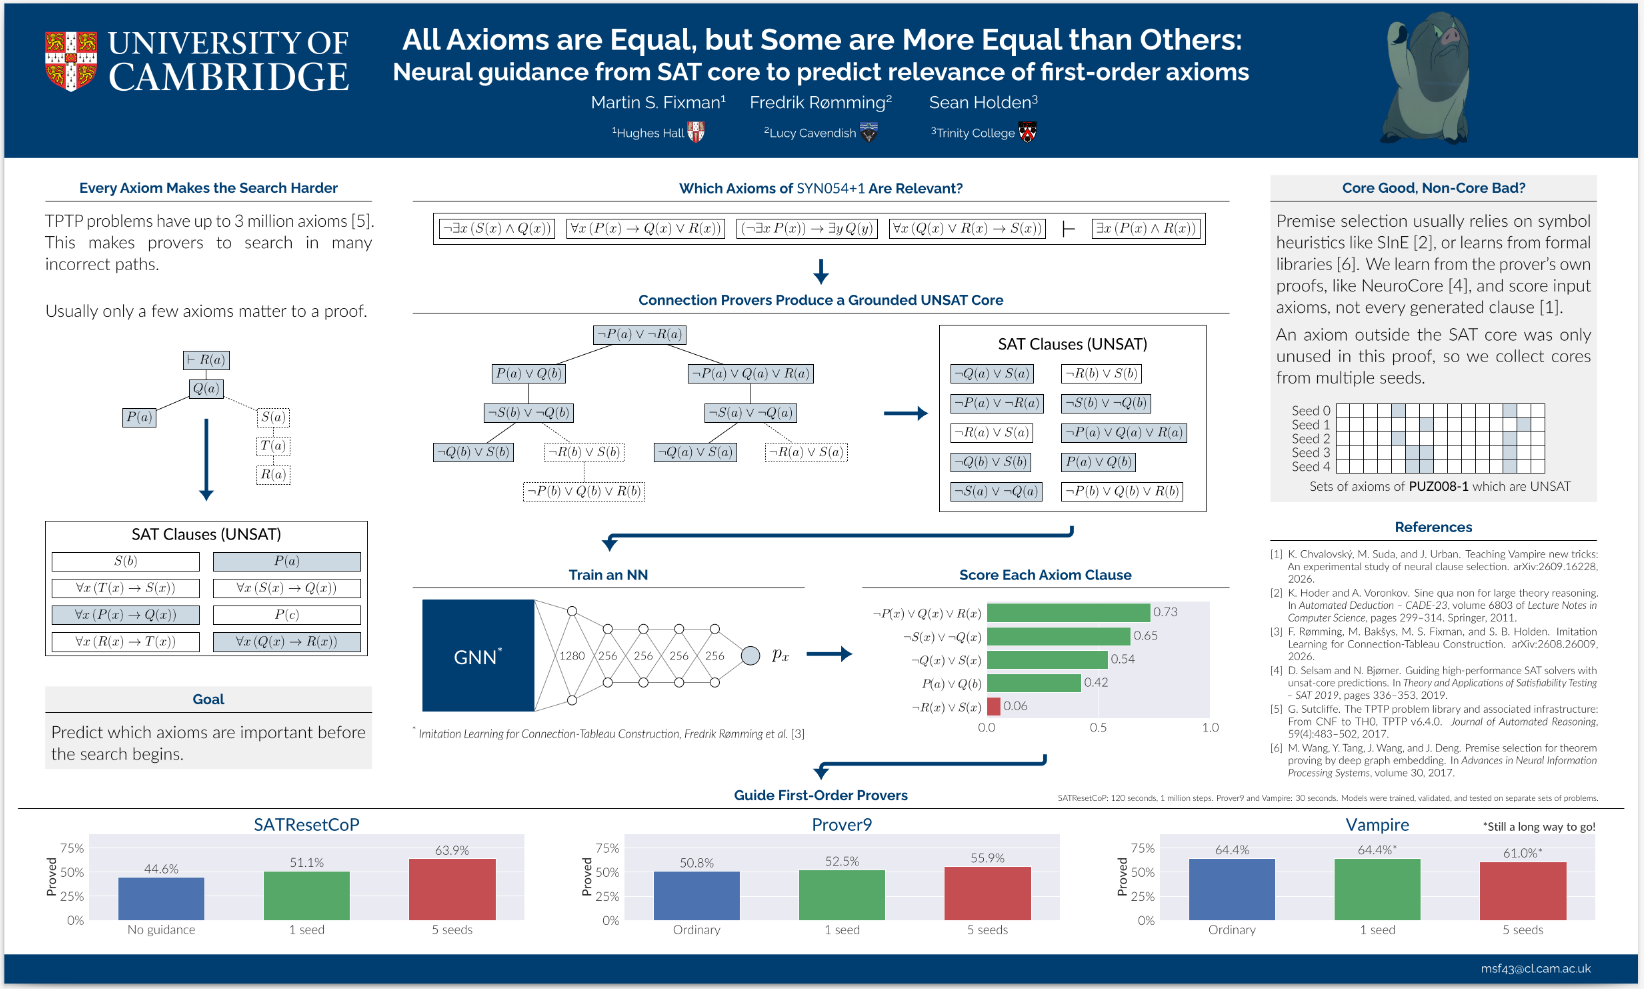
\includegraphics[height=200pt]{poster.png}
	\caption{Updated version of the poster presented to the CST poster session.}
	\label{poster}
\end{figure*}

I presented a poster in the CST session last Tuesday.
It had a good reception due to the good ration of graphics compared to text, and it was simple understand to let people not familiar with ATPs to understand this topic.

The main criticism of the poster was that it was hard to understand, without an explanation, what problem I was trying to solve in the first place.
The poster in \cref{poster} is the corrected version with this added.


\section{Improvements to Pre-training}

I settled on using the \cop{ExtraLargeFull} model, trained on both \cop{SATCoP} and \cop{SATResetCoP} data.
I also built the following improvements to the axiom selector.

\subsection{Collecting Multiple Seeds}

Both \cop{SATCoP} and \cop{SATResetCoP} have a high level of randomness in them, and can produce many different unsatisfiability proofs with different UNSAT cores from the same problem.

One of the ideas that came up last week was running \texttt{axiom\_predictor.py} collected on several seeds.
This helps in two ways.
\begin{enumerate}
	\item There are more UNSAT cores to train from.
	\item Many important axioms don't get negative samples due to not being part of the solution given by either model.
\end{enumerate}

Following the medieval theme in these models I am calling this set of models \cop{Sharbaraz\{e\}}, for the model trained with seeds $0$ to $e - 1$.

\newpage

\subsection{Joining step}

\begin{table}[h]
	\centering
	\scriptsize
	\setlength{\tabcolsep}{4pt}
	\begin{tabular}{lrrrrr}
		\toprule
		& \multicolumn{2}{c}{Examples} & \multicolumn{2}{c}{Axioms (millions)} & \\
		\cmidrule(lr){2-3} \cmidrule(lr){4-5}
		& Pre-join & Post-join & Pre-join & Post-join & Training \\
		\midrule
		\cop{Sharbaraz1} & \num{10601} & \num{10449} & \num{11.5} & \num{11.5} & \qty{114}{\minute} \\
		\cop{Sharbaraz5} & \num{53033} & \num{23571} & \num{57.1} & \num{31.9} & \qty{264}{\minute} \\
		\cop{Sharbaraz10} & \num{106307} & \num{35230} & \num{114.5} & \num{48.0} & \qty{402}{\minute} \\
		\cop{Sharbaraz15} & \num{159554} & \num{45049} & \num{172.2} & \num{61.5} & \qty{516}{\minute} \\
		\cop{Sharbaraz20} & \num{212908} & \num{54004} & \num{229.9} & \num{74.3} & \qty{570}{\minute} \\
		\bottomrule
	\end{tabular}
	\caption{We are training from a large amount of data. Collection attempted \num{17436} problems from \num{10871} families.}
	\label{join_table}
\end{table}

\begin{figure}[h]
	\scriptsize
	\begin{subfigure}[t]{.47\columnwidth}
		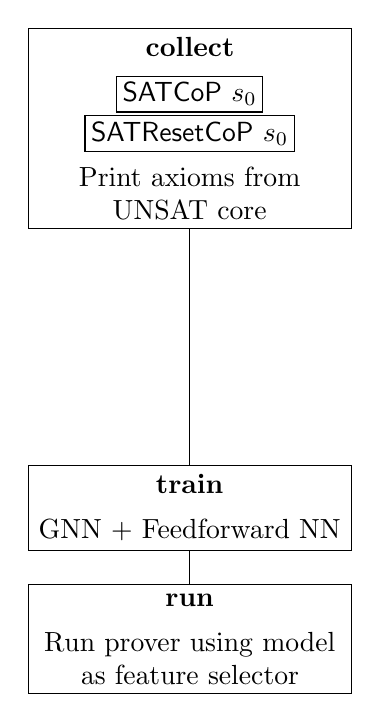
\begin{tikzpicture}[box/.style = {draw, align = flush center, text width = 110pt}, node distance = 12pt]
			\node[box] (collect) {\textbf{collect} \\[1ex] \fbox{\cop{SATCoP} $s_0$} \fbox{\cop{SATResetCoP $s_0$}} \\[1ex] Print axioms from UNSAT core};
			\node[box, below = 85pt of collect] (train) {\textbf{train} \\[1ex] GNN + Feedforward NN};
			\node[box, below = of train] (run) {\textbf{run} \\[1ex] Run prover using model as feature selector};

			\draw (collect) -- (train);
			\draw (train) -- (run);
		\end{tikzpicture}
		\caption{The old version of the trainer only used one seed per model.}
		\label{diagram_left}
	\end{subfigure}\hfill
	\begin{subfigure}[t]{.49\columnwidth}
		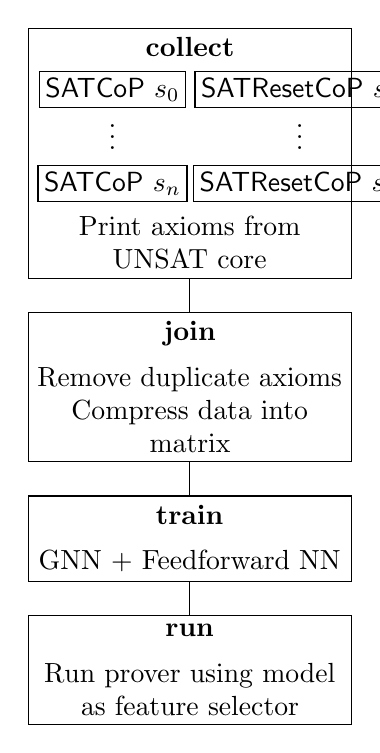
\begin{tikzpicture}[box/.style = {draw, align = flush center, text width = 110pt}, node distance = 12pt]
			\node[box] (collect) {\textbf{collect} \\[1ex] {
				\begin{tabular}{@{}c@{\hspace{2pt}}c@{}}
					\fbox{\cop{SATCoP} $s_0$} & \fbox{\cop{SATResetCoP} $s_0$} \\
					\vspace{1pt}\vdots & \vspace{1pt}\vdots \\
					\fbox{\cop{SATCoP} $s_n$} & \fbox{\cop{SATResetCoP} $s_n$}
				\end{tabular}
				% \fbox{\cop{SATCoP} $s_0$} \fbox{\cop{SATResetCoP $s_0$}}
			} \\[1ex] Print axioms from UNSAT core};
			\node[box, below = of collect] (join) {\textbf{join} \\[1ex] Remove duplicate axioms \\ Compress data into matrix};
			\node[box, below = of join] (train) {\textbf{train} \\[1ex] GNN + Feedforward NN};
			\node[box, below = of train] (run) {\textbf{run} \\[1ex] Run prover using model as feature selector};

			\draw (collect) -- (join);
			\draw (join) -- (train);
			\draw (train) -- (run);
		\end{tikzpicture}
		\caption{The new version uses multiple seeds per model, and later removes duplicate axioms to accelerate training.}
		\label{diagram_right}
	\end{subfigure}
	\caption{Axiom selector actions before \textbf{(a)} and after \textbf{(b)} the new \texttt{join} action.}
	\label{what_do}
\end{figure}

\begin{wrapfigure}{r}{80pt}
	\centering
	\vspace{-10pt}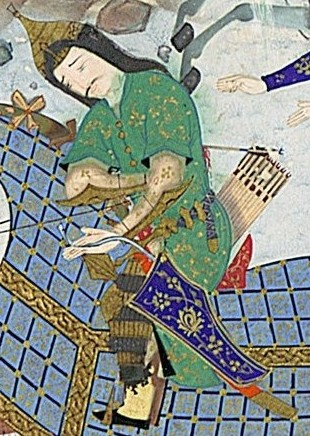
\includegraphics[width=50pt]{Sharbaraz.jpg}
	\caption*{Sharbaraz, the boar of the (Sassanian Persian) Empire, who conquered the Middle East in the 7th century.\vspace{-40pt}}
\end{wrapfigure}

Having a large amount of possibly repeated seeds made training much slower, so I remove duplicates as a new step between \texttt{collect} and \texttt{train}.
I also transform the format from a \texttt{csv} to a PyTorch-optimised compressed matrix.

This makes training considerably faster, and prevents me from going over the space limit the RDS partition in the HPC.

\Cref{what_do} shows a rough diagram of the steps to train a model and run it, while \cref{join_table} shows the size difference between different models.

\section{Training}

Five different models were trained with seeds from 1, 5, 10, 15, and 20 different runs using the same train/validation/test split as before.
\Cref{join_table} shows that the training took relatively little GPU time, which is an improvement for rapid training.

\begin{figure}[h]
	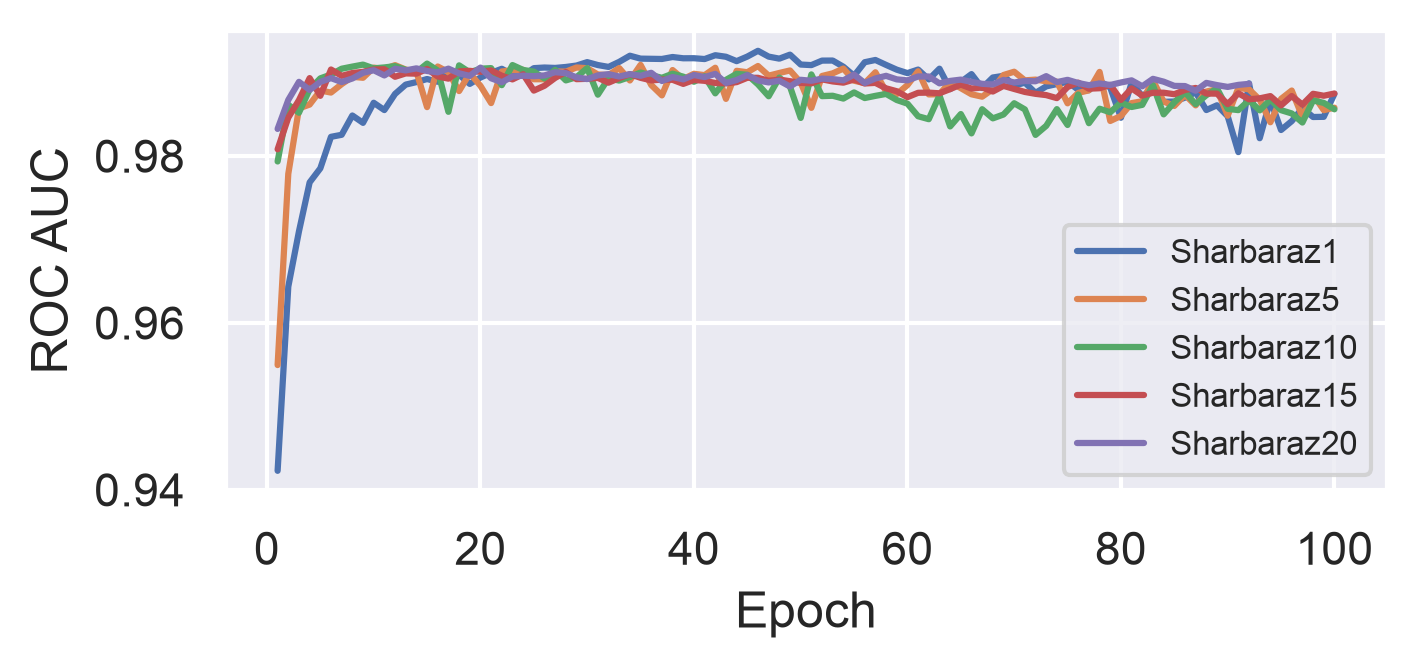
\includegraphics[width=\columnwidth]{roc_auc.png}
	\caption{The validation ROC AUC of all models maxes out after only a few epochs. This is a good sign.}
	\label{roc_auc}
\end{figure}

\Cref{roc_auc} shows that the ROC AUC maximises (at a very high level) around epoch 10 for all models but \cop{Sharbaraz1}.
However, since these models will have a non-trivial that's not closely related to the training data the epoch with the highest ROC AUC might not be the best epoch for the final result.

To settle this, I ran the models on guided versions of \cop{SATCoP} and \cop{SATResetCoP} for all 1777 TPTP problems in the validation set to find which one has the best result.

\begin{figure}[h]
	\begin{subfigure}{\columnwidth}
		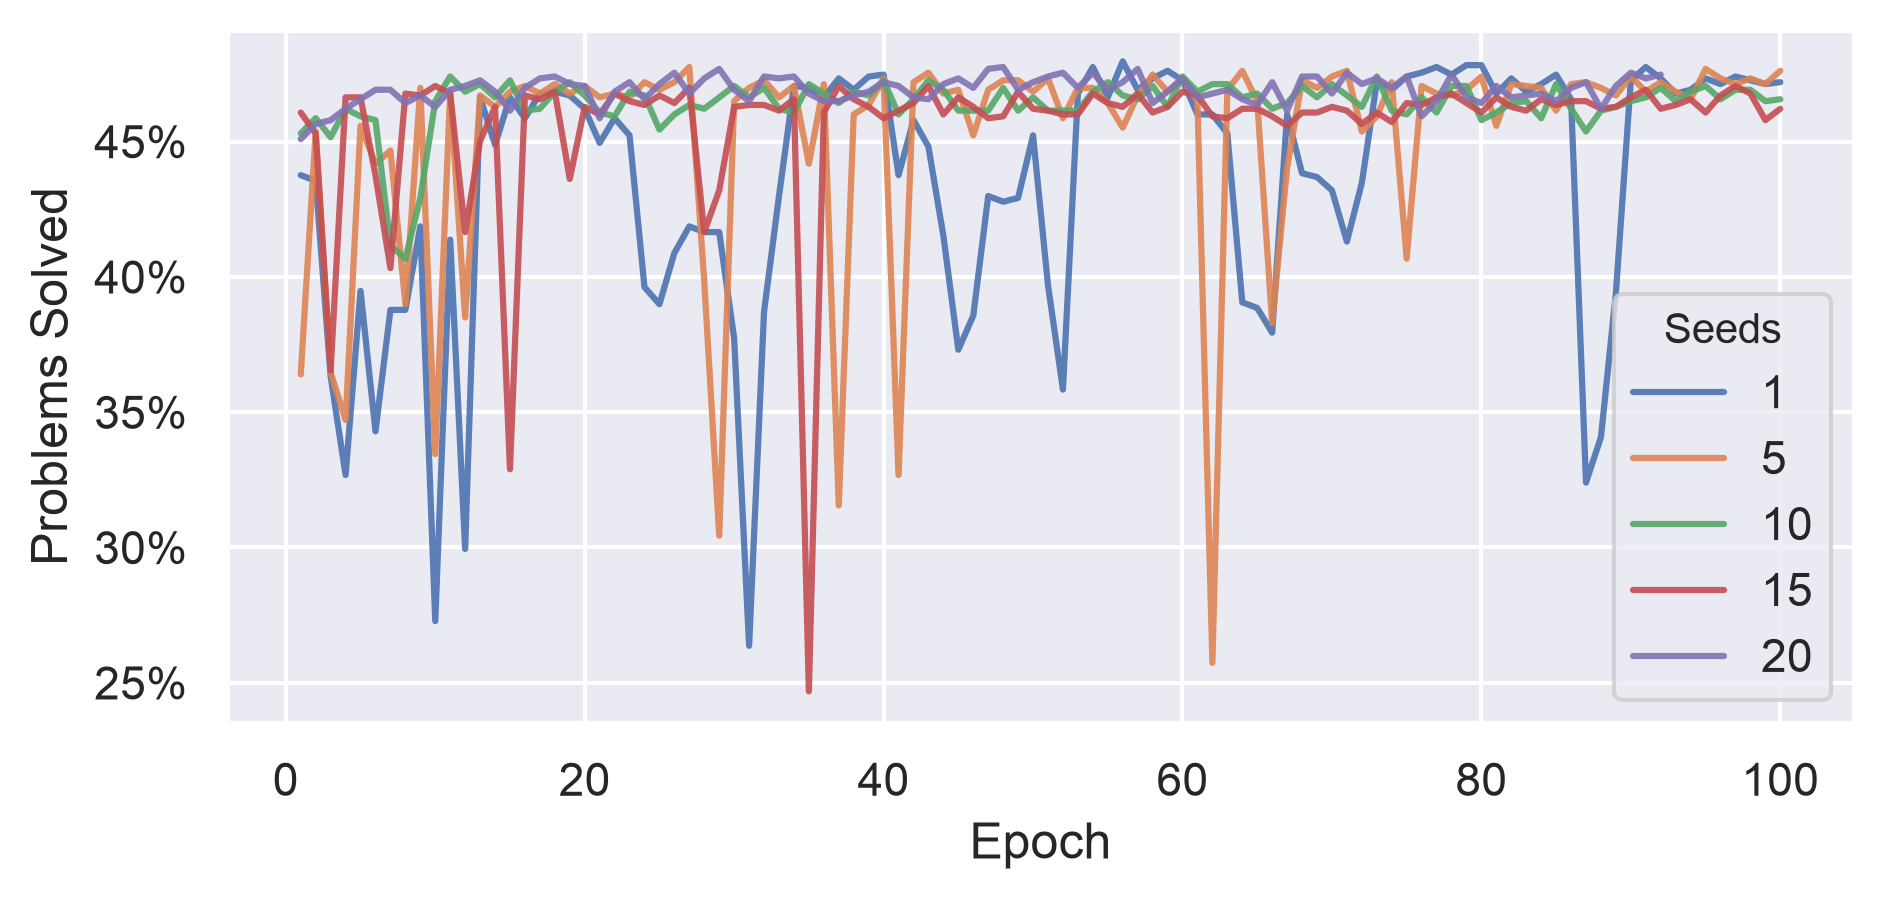
\includegraphics[width=\columnwidth]{satcop_epochs.png}
		\caption{Results on \cop{SATCoP}. The results are spiky due to training issues (this is normal), but there is little improvement in continuing training after around epoch 20.}
	\end{subfigure}
	\begin{subfigure}{\columnwidth}
		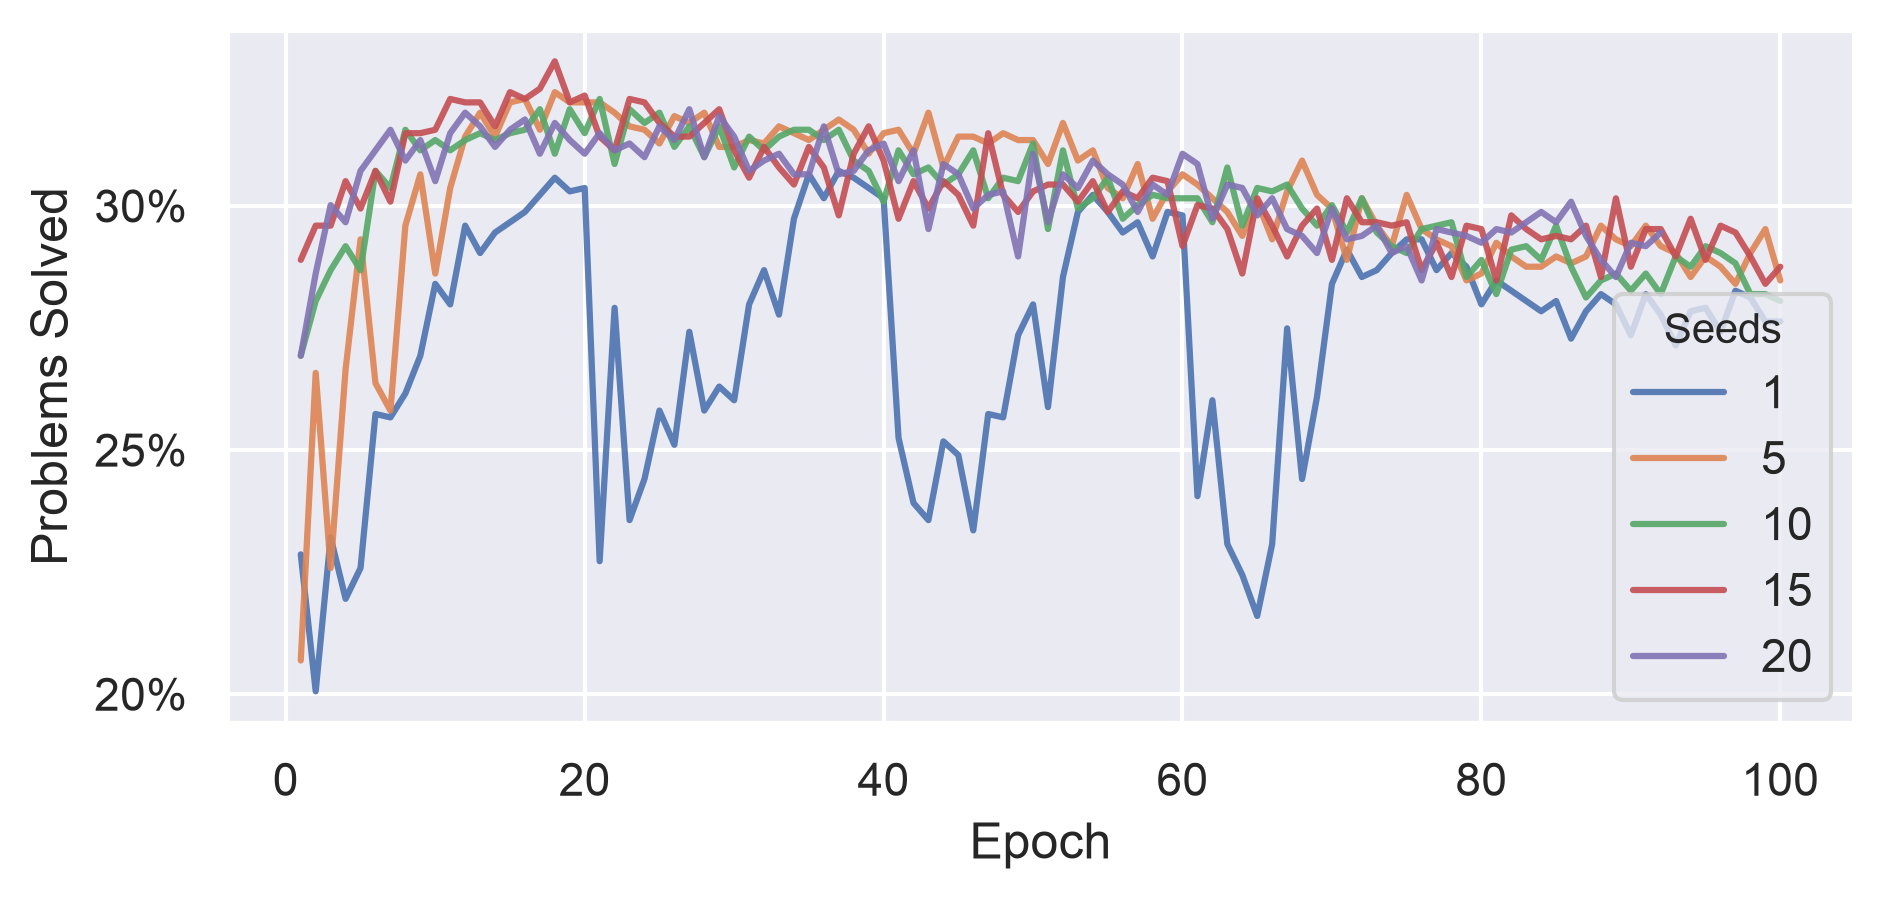
\includegraphics[width=\columnwidth]{satresetcop_epochs.png}
		\caption{Results on \cop{SATResetCoP}. The results for all trainers actually start overfitting and become \textit{worse} on successive epochs, and overall they are less spiky than in \cop{SATCoP}.}
	\end{subfigure}
	\caption{Results of running each epoch of each seed on both \cop{SAT\*} provers. The axiom predictor uses weighted sampling to guide these two models.}
	\label{validation_results}
\end{figure}

\Cref{validation_results} shows that the validation set acts very differently on both \cop{SATCoP} and \cop{SATResetCoP}.

I spent some time investigating whether this was due to a bug, and at this point I am convinced that it's due to the properties of both provers.
Since \cop{SATResetCoP} resets more often, a bad initial seed (which is more common on overfit trainers) will have a worse overall performance.

For the following experiments I decided to use \cop{Sharbaraz5} and \cop{Sharbaraz15}, both on Epoch 20.
This will be changed afterwards, since this model could use a good hyperparameter sweep before re-running the next experiments.

\section{Results}

\subsection{Provers}
\label{provers}

Rather than creating our own fake comparison provers, like Fixman~et~al.\ did in his seminal paper\cite{satresetcop}, I am testing this on the canonical version of the following provers.
\begin{description}[itemsep=0pt]
	\item[\cop{Prover9}] \url{https://www.cs.unm.edu/~mccune/prover9/}
	\item[\cop{E}] \url{https://github.com/eprover/eprover}
	\item[\cop{SPASS}] \url{https://www.spass-prover.org/}
	\item[\cop{iProver}] \url{https://gitlab.com/korovin/iprover}
	\item[\cop{Vampire}] \url{https://github.com/vprover/vampire}
\end{description}

I cannot easily modify them to add a weighted sampling like I did with \cop{SATCoP}, so instead I run them inside a container that runs the following steps.

\begin{enumerate}
	\item Run the \cop{Sharbaraz} model, score all axioms.
	\item Keep only the $n$ axioms with the highest scores, with $n$ defined by the portfolio.
	\item Run the model on these $n$ axioms.
\end{enumerate}

This is doable without modifying the source code of any of the other models.

\subsection{Portfolios}
\label{portfolios}

I borrow an idea from the DeepMath paper from Irving~et~al\. (including Josef~Urban)\cite{deepmath}, and use two different portfolios to control 

\begin{description}
	\item[1. Simple Portfolio] \phantom{a}
		\begin{enumerate} 
			\item Score all the axioms.
			\item Top 16 axioms 8 seconds.
			\item Base model until time out.
		\end{enumerate}
	\item[2. Complex Portfolio] \phantom{b}
		\begin{enumerate}
			\item Score the axioms.
			\item Top 16 axioms 8 seconds.
			\item Top 64 axioms 8 seconds.
			\item Top 256 axioms 8 seconds.
			\item Base model until time out.
		\end{enumerate}
\end{description}

\subsection{Results}

Each of the 2 portfolios from \cref{portfolios} is run on each of the provers from \cref{provers} on the HPC with a 60 second time limit using the test data (part 9, the problems from \sfrac{1}{10}th of the TPTP problem families).

\begin{table}[h]
	\centering
	\scriptsize
	\setlength{\tabcolsep}{2pt}
	\begin{tabular}{lcrr@{\hspace{12pt}}rr@{\hspace{6pt}}rr}
		\toprule
		Model & Method & \cop{SATCoP} & \cop{Prover9} & \cop{iProver} & \cop{SPASS} & \cop{E} & \cop{Vampire}\footnotemark{} \\
		\midrule
		\multirow{3}{*}{\cop{Sharbaraz5}} & Base & \num{692} & \num{379} & \num{414} & \num{347} & \num{468} & \num{957} \\
		& \textbf{(1)} & \num{699} & \num{394} & \num{414} & \num{348} & \num{468} & \num{944} \\
		& \textbf{(2)} & \num{710} & \num{403} & \num{416} & \num{348} & \num{468} & \num{954} \\
		\midrule
		\multirow{3}{*}{\cop{Sharbaraz15}} & Base & \num{692} & \num{378} & \num{412} & \num{347} & \num{468} & \num{951} \\
		& \textbf{(1)} & \num{699} & \num{396} & \num{416} & \num{348} & \num{467} & \num{942} \\
		& \textbf{(2)} & \num{712} & \num{401} & \num{418} & \num{349} & \num{467} & \num{949} \\
		\bottomrule
	\end{tabular}
	\caption{Problems proved on the test set. \cop{SATCoP} and \cop{Vampire} run on \num{1426} problems; the other provers run on \num{608} CNF problems.}
	\label{pareto_table}
\end{table}

\footnotetext{I am currently running Vampire \textit{without} SInE\cite{hoder2011sine}, since the results are not good anyway. If I ever beat this baseline I will start using SInE as a new baseline.}

The results in \cref{pareto_table} show significant improvements in \cop{SATCoP} and \cop{Prover9} with the second portfolio (2.9\% and 6.3\% respectively), along with a \textit{tiny} improvement in \cop{E}, \cop{SPASS}, and \cop{iProver} and no improvement at all on Vampire.

There does not seem to be any significant difference between the 5-seed and the 15-seed version, which is consistent with the results in \cref{validation_results}: as long as the right epoch is chosen, the results with more than 1 seed tend to be the same despite training with over 30 thousand extra examples.

\section{Next Steps and Experiments}

\subsection{Improving the Models}

I will run a hyperparameter sweep to improve the model, and possibly experiment a bit with different architectures.
I believe there is a bit of extra juice I can take from this.

\subsection{Subutai: training on other provers}

\begin{wrapfigure}{r}{80pt}
	\centering
	\fbox{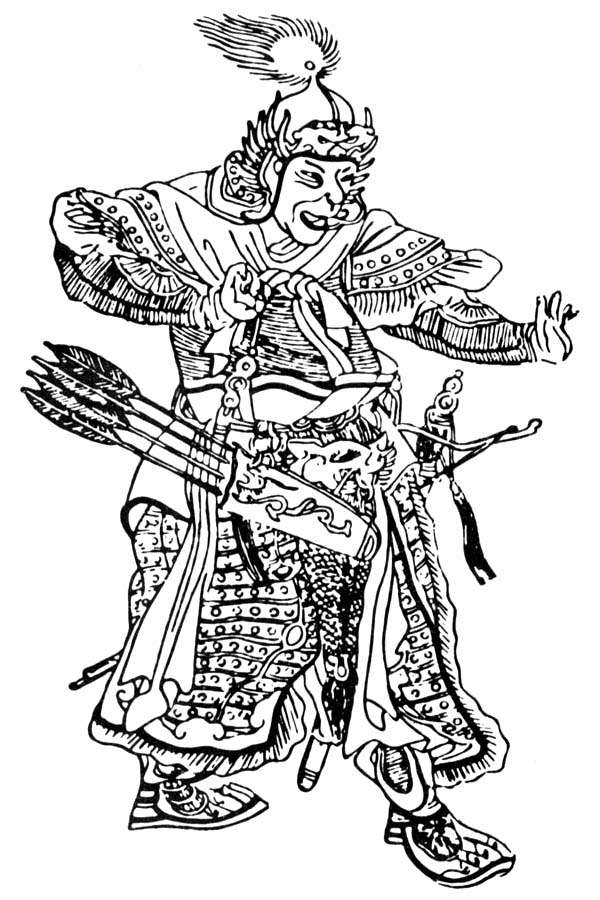
\includegraphics[width=50pt]{Subutai.jpg}}
	\caption*{Subutai, the scourge of the world, who conquered all of Central Asia.}
\end{wrapfigure}

The models seem to be particularly good on \cop{SATCoP} and \cop{SATResetCoP}, and a bit better but still worse on \cop{Prover9} and other provers.
I am currently in the process of training a new set of models, named after the 13th century Mongol general \cop{Subutai}, which train on the output data of different provers. 

I have some home that these will have better results on their particular provers.
If so, it's worth it moving this experiment to training the axiom scorer on the prover that's going to be used in; this might be a good experiment.

\subsection{So... where do I publish this?}

Is this publishable? Assuming the \cop{Subutai} experiments don't improve out results much, the improvements are modest compared to any of the ``good'' provers.

There are a few novel ideas, and I was aiming for one of these conferences.
\begin{description}
	\item[IJCAI] Deadline 11 January, conference early August in Kyoto.
	\item[CADE] Deadline 22 February, conference late August 2027 in Nijmegen (I'm publishing something here regardless)
	\item[AITP] Deadline May, you know when and where it is.
\end{description} 

Do you think this is enough? Or should I just work on something else and maybe fill this here?

\printbibliography{}

\end{document}
